\chapter{Data}
\label{cha:data}

This chapter contains a description of the two datasets used, together with the preprocessing steps and a description of how the data was represented.
It also provides a more in-depth analysis of the relationship between certain aspects of the clinical dataset and the topics generated by an LDA model.
These relationships perform the basis for some of the decisions made in Chapter~\ref{cha:experiments}, and will be discussed in Chapter~\ref{cha:discussion}.

\section{Datasets}\label{sec:datasets}

Two different datasets were used in this thesis.
They were the dataset of clinical reports provided by Sectra, as well as Reuters-21578 \footnote{Reuters-21578, https://archive.ics.uci.edu/ml/datasets/reuters-21578+text+categorization+collection}.
The latter was used in order to be able to simulate a multi-label labeling process.
Before being integrated into Sectra's system, the different active learning strategies needed to be evaluated from an objective point of view, so that any tradeoffs were known beforehand.
Since the vast majority of the dataset from Sectra was unlabeled, this could not effectively have been done using only that.
In order to simulate an annotator labeling reports, the unlabeled pool must consist of data points for which a label can be automatically retrieved.
Since the Sectra dataset had only had 500 assigned labels, this would not have provided as much insight as the Reuters-21578 dataset.

\subsection{Clinical Dataset From Sectra}

The set of reports provided by Sectra contained 1 068 904 different entries, where 493 were initially labeled.
The entries were spread out over several files and stored in the JSON format.
However, those labels were subject to change, so they were mainly used to see if there was a correlation between the labels and clusters during the exploration phase.
A sample report can be seen in Figure~\ref{fig:sample-report}.
The fields include:
\begin{enumerate}
    \item \textbf{ExamId}: The ID of the exam.
    \item \textbf{ReportText}: The text for the report written by the physician after the examination.
    \item \textbf{Anamnesis}: The patient's medical history.
    \item \textbf{PatientAlert}: Anything special about the patient.
    \item \textbf{ExamComment}: Comments regarding the performed examination.
    \item \textbf{Cancelled}: Whether or not the examination was Cancelled.
    \item \textbf{ExamName}: Name of the exam.
    \item \textbf{ExamCode}: Code for the exam.
    \item \textbf{PatientSex}: The sex of the patient.
    \item \textbf{PatientAge}: Age of the patient. This field is truncated if it is above 90 years.
    \item \textbf{Urgent}: If the examination is urgent or not.
    \item \textbf{Pharma}: List of administrated pharmaceuticals.
\end{enumerate}
\begin{figure}
\begin{verbatim}
    {
        'ExamId':       3302250, 
        'ReportText':   '[NUM-SEQ] 
                        Craniell datortomografi utan och med 
                        intravenös kontrast:
                        
                        Frontalt på höger sida finns ett c:a 
                        4 x 3 cm stort lågattenuerande område, tolkas 
                        representera rest efter genomgången 
                        parenchymskada, troligen äldre kontusionsblödning. 
                        Subcorticalt på ömse sidor om centralfåran på 
                        höger sida finns ett några cm-stort 
                        lågattenuerande område som kan vara ischemiskt. 
                        Lätt sänkt attenuering av vit substans 
                        periventrikulärt förenlig med leuko-araios av 
                        degenerativ natur. För åldern normalstora 
                        ventriklar. Corticala sulci upp mot konvexiteten 
                        är något smalare än förväntat för åldern. 
                        
                        Någon tumörsuspekt förändring påvisas ej.',
        'Canceled':     False, 
        'Question':     'Förändring vä temporalt?',
        'PatientAlert': 'Hepatit C-positiv.', 
        'ExamComment':  "Alla kontrastfrågor: UA mnn", 
        'ExamName':     'DT hjärna utan och med iv kontrast',
        'Anamnesis':    'Pat med skalltrauma på 60-talet. Kommer nu med 
                        nattliga från-varoattacker. Skrikigt beteende 
                        som tolkats som epilepsi. CT är aldrig gjort. 
                        HEPATIT C-positiv."',
        'ExamCode':     '81081', 
        'PatientSex':   'MALE', 
        'PatientAge':   59, 
        'Urgent':       0, 
        'Pharma':       [{"ExamId": 3200240, "Units": "100 ml", 
                        "Pharma": "Omnipaque Inj.lösn 300 mg I/ml"}]
    }
\end{verbatim}
\caption{A sample report from the dataset provided by Sectra}
\label{fig:sample-report}
\end{figure}

The work was mainly concerned with the ReportText field, since it contains the response to the result of the examination.
But for the complete active learning system the Anamnesis field was used as well, since it provides important patient information.
The labels that were initially assigned to these reports were:
``Blödning'', ``Infektion'', ``Metabol'', ``Tumör'', ``Cysta'', ``Missbildning'', ``Syndrom'', ``Demens'', ``Hydrocefalus'', ``Infarkt'', ``Kärlsjukdom'', ``Trauma'', ``Systemsjukdom'', ``Inklämmning'' and ``Normal''.
The distribution of categories among these initially labeled reports can be seen in Figure~\ref{fig:class-distribution}.
Note that this is only a count of the different labels.
The plot is therefore disregarding which labels occurred together.

\begin{figure}
    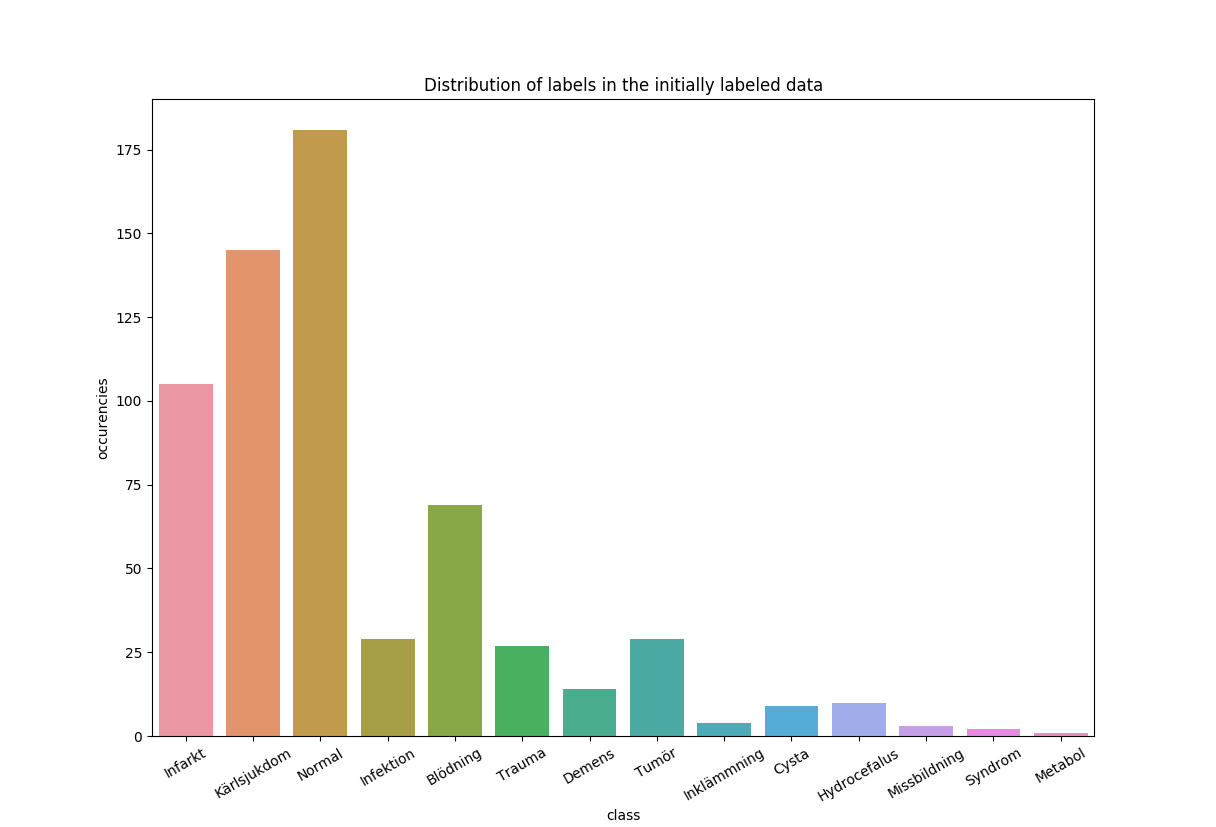
\includegraphics[width=\textwidth]{figures/class-distribution.png}
    \caption{The distribution over the labels in the initial set of labeled data provided by Sectra}
    \label{fig:class-distribution}
\end{figure}

\subsection{Reuters-21578}

The Reuters-21578 newswire dataset is widely used when it comes to text classification research and provides a good multi-label benchmark that can be used to compare how well certain techniques perform to other papers.
It is a set of news stories, so there is only one text data field.
All experiments used the \textit{ModApte} split of the dataset, which is commonly used and readily available.
It splits the dataset into a predefined set of training and test documents, containing 7769 and 3019 entries respectively.
This split contains a subset of the categories, specifically 90 different ones.
Since the clinical dataset from Sectra only contained 15 different categories, this would not mirror that very well, so instead the 15 most common categories of those were taken out.
The 15 most common categories were (in order of label count): ``earn'', ``acq'', ``money-fx'', ``grain'', ``crude'', ``trade'', ``interest'', ``wheat'', ``ship'', ``corn'', ``money-supply'', ``dlr'', ``sugar'', ``oilseed'' and ``coffee''.
The distribution of the top 15 Reuters-21578 categories can be seen in Figure~\ref{fig:class-distribution-reuters}.
After filtering out the documents not labeled with any of the top 15 categories, there were 6880 documents left in the training set, and 2646 in the test set.

\begin{figure}
    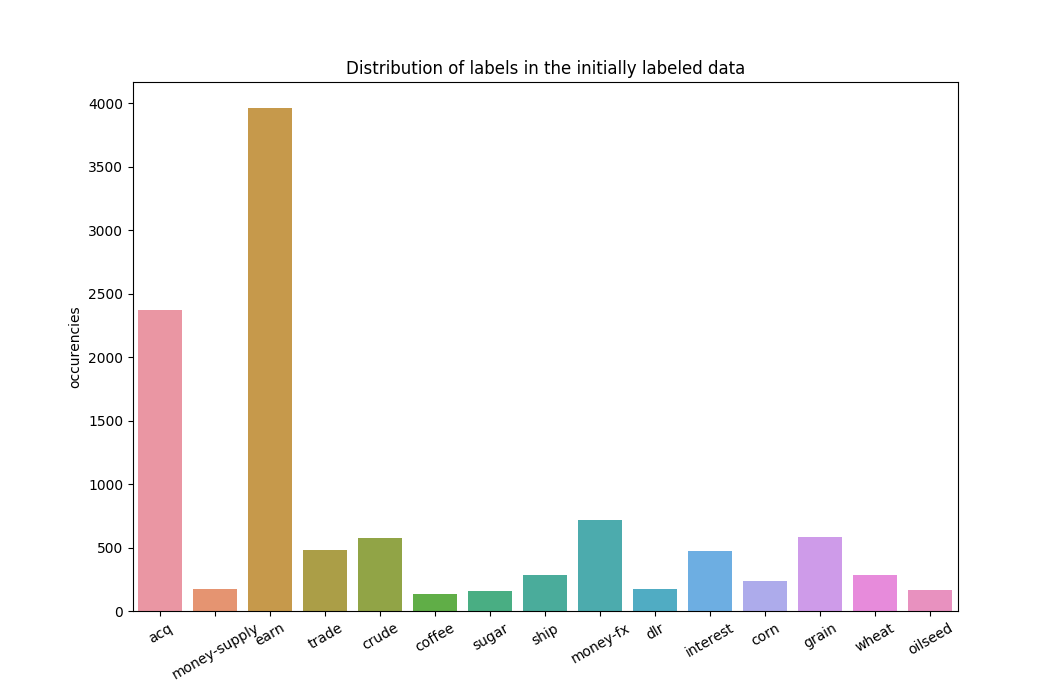
\includegraphics[width=\textwidth]{figures/class-distribution-reuters.png}
    \caption{The distribution over the labels in the Reuters data}
    \label{fig:class-distribution-reuters}
\end{figure}

\section{Pre-Processing and Text Representation}\label{sec:pre-processing}

Before the data was used in the conducted experiments, several pre-processing steps were applied in order to clean the dataset and make it easier to work with.
They were:
\begin{enumerate}
    \item The first step was to extract the fields of interest.
          For the exploratory phase, and for the use of active learning techniques these were ``ReportText'' and ``Anamnesis''.
          When it came to filtering out invalid reports, the ``ReportText'' was the only field of concern.
          It describes the results of the examination, and therefore if there was an examination at all.
    \item White space and punctuation were stripped from the data.
    \item All words were transformed into lowercase.
    \item \label{enum:step-4} The most common words, as well as very infrequent words, were both filtered out.
          Specifically, words occurring in less than 1\% of the documents, and words occurring in more than 90\% were removed.
          The idea behind this is that these words would not contribute to differentiating different classes of documents.
          Removing of both frequent and infrequent words is commonly done when working with text and has been done in the context of classification, active learning or topic modeling before~\cite{tong2001support, blei2003latent, brinker2006active, sarioglu2013topic}.
    \item A list of identified common stopwords was removed as well.
          Stopwords are words that are not deemed to be of significance.
          This list of words was based on the Swedish nltk stopwords list.
          After iterating over the dataset, words that occurred frequently but were not considered to be very informative for the models were identified.
          The list of stopwords was then extended to incorporate these words as dataset-specific information.
          For example, this included names of the doctors that had written the report.
          By removing names of doctors the idea is to make the system more applicable to new reports, written by other doctors.
    \item Accents from the words were removed.
    \item The text was tokenized and then stemmed using the Swedish Porter2 stemmer \footnote{Swedish Porter Stemmer, http://snowball.tartarus.org/algorithms/swedish/stemmer.html}.
          Stemming is the task of making words of different plurality and tense into a common base form.
\end{enumerate}
Most of these steps have been performed in previous research  dealing with text analysis in the form of classification or active learning~\cite{tong2001support, blei2003latent, brinker2006active, sarioglu2013topic}.


Identifying synonyms and names that could be added to the stopwords was done with a word2vec model.
A word2vec model was used on the entire dataset to analyze the relationship between terms and to find possible synonyms.
In order to find synonyms, all words in the dataset that according to the word2vec model had a similarity over 95\% were manually inspected.
By doing this, 420 pairs were discovered.
The vast majority of these were words that are used in similar contexts, which includes opposites like ``left'' and ``right'', and some names.
Some of the medical terms were hard to interpret and were therefore not considered to be synonyms.
Disregarding these, the synonyms and misspellings that were decided to be used in the final system can be seen in Table~\ref{tab:synonyms}.
The original value was replaced with the new one during the preprocessing stage.

\begin{table}
    \centering
    \begin{tabular}{|ccc|}
        \hline
        \textbf{Original} & \textbf{Replacement} & \textbf{Type} \\
        \hline
        ordinärt & normalt & synonyms \\
        ej & inte & synonyms \\
        avbeställd & avbokad & synonyms \\
        avebställd & avbokad & misspelling + synonym \\
        belsutat & beslutat & misspelling \\
        måttliga & lätta & synonyms \\
        pat & patient & short \\
        pt & patient & short \\
        pateint & patient & misspelling \\
        akuten & akutmottagningen & synonym \\
        us & undersökning & short \\
        \hline
    \end{tabular}
    \caption{The synonyms, misspellings and shorts found in the data that the author could assert with confidence.}
    \label{tab:synonyms}
\end{table}

In addition to finding synonyms, this model was used to identify names and other identifiers in the reports.
They would come up as similar entities by the model since they are often used in the same context.
In order to visualize the data in a 2D plot, t-distributed stochastic neighbor embedding (t-SNE) was used.
It is a dimensionality reduction technique, that is able to transform high dimensional data into two dimensions while working to retain as much variance as possible.
For the purpose of identifying names, a key insight was that most of the names in the medical reports were used in very similar contexts.
Usually, it was a doctor providing a signature to the examination.
Since names are commonly used in similar contexts, they have similar attributes in the word embedding model.
Given that the names got similar coordinates in the plot, identifying the section with names allowed for the identification of a lot of the names used in the reports.
Figure~\ref{fig:word2vec-names-overview} shows how this was used to identify a group of names.
This is unlikely to catch all of the names, but a lot of them.
Very uncommon names will be filtered out by step~\ref{enum:step-4} in the preprocessing steps outlined above.

\begin{figure}
    \begin{subfigure}[b]{\textwidth}
        \centering
        \fbox{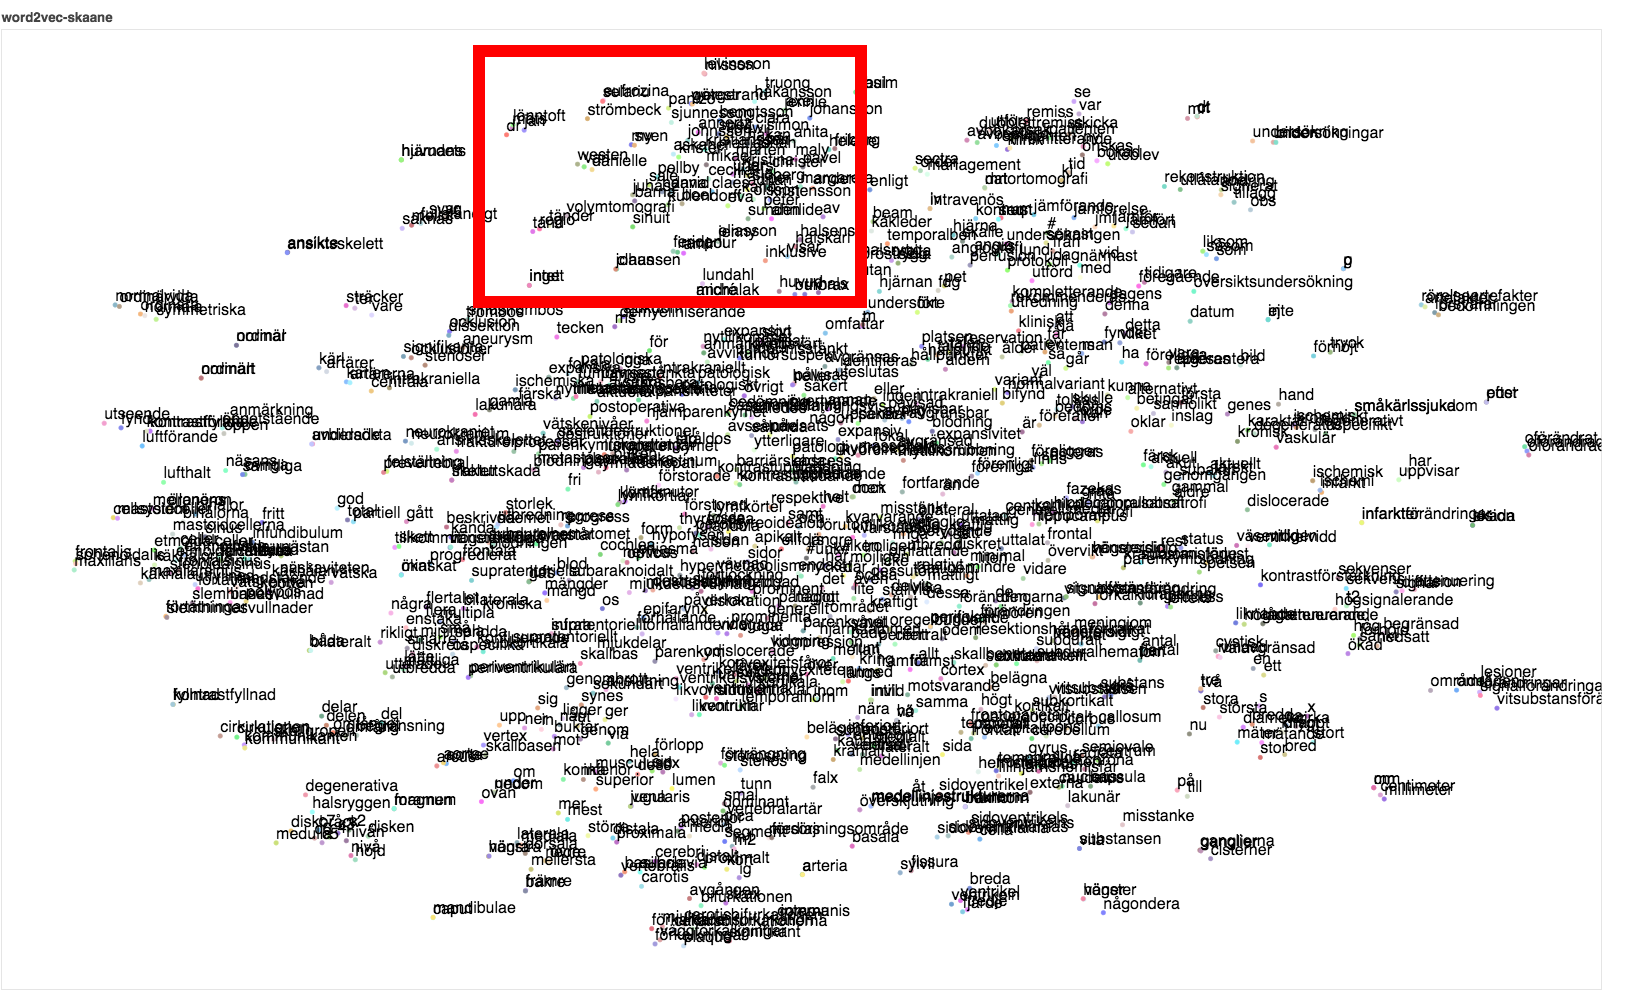
\includegraphics[width=\textwidth]{figures/word2vec-overview.png}}
        \caption{A 2D plot of the full word2vec model.}
    \end{subfigure}
    \quad
    \begin{subfigure}[b]{\textwidth}
        \centering
        \fbox{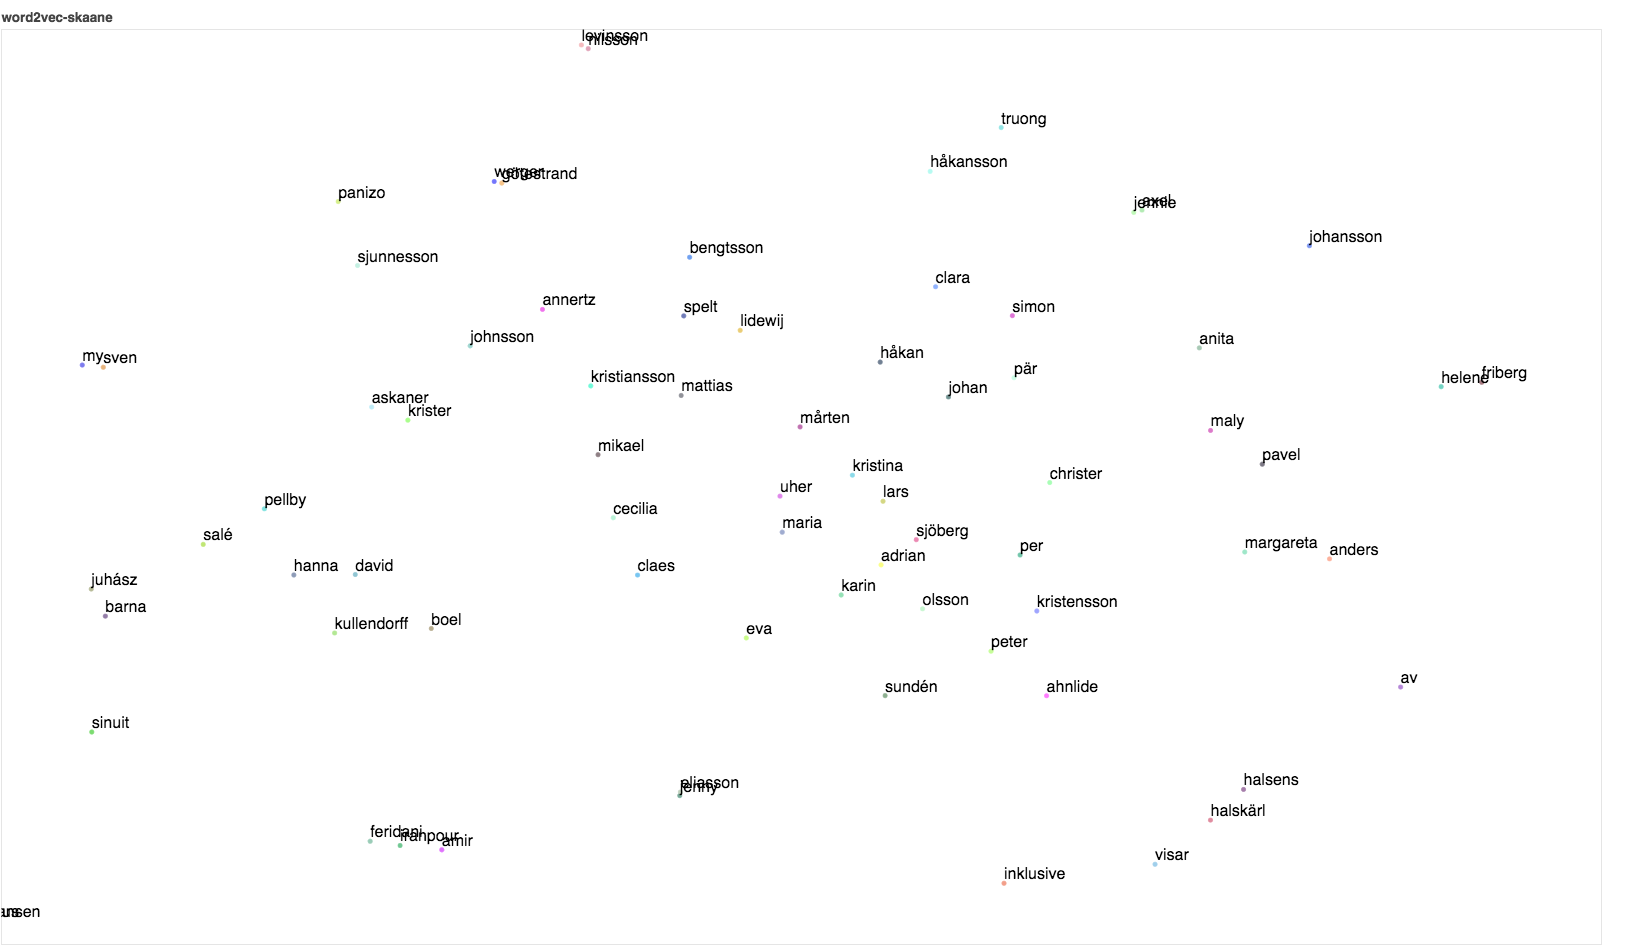
\includegraphics[width=\textwidth]{figures/word2vec-names.png}}
        \caption{A 2D plot of the subset of the word2vec model covering the names.}
    \end{subfigure}
    \caption{Two figures illustrating how the names were discovered in the word2vec plot. The (b) plot represents the red square in (a).}
    \label{fig:word2vec-names-overview}
\end{figure}


After transforming the text into a sequence of tokens, the final step before using it with the models was to create a representation that would be beneficial to work with.
The representation chosen was bag of words, i.e. a matrix of tokens count.
Each document is represented by the counts of each token, disregarding the order of the tokens.
In order to get some positional information into the representation, additional tokens are stored. 
The additional tokens are bigrams, which are pairs of tokens (i.e. processed words).
By storing the frequency of how often such a pair occurs in the document, alongside the regular one-word tokens, some positional information is retained.

\section{Exploratory Study}\label{sec:exploratory-study}

For the exploratory study, the representation described in Section~\ref{sec:pre-processing} was used.
The goal of this phase was to acquire a better understanding of the data, how it was structured and what kind of information might be extracted from it.
A part of this goal was to go through the fields for the different reports to see how they worked and what values could be expected.
Certain fields such as the canceled field did not seem to be very reliable. 
Reports that clearly explained a situation where the patient had been transferred to another hospital, or for another reason not having performed an examination, still described a situation where the canceled field was set to ``false''.
This is treated in research question~\ref{intro:re-q3}.

The first step was to fit an LDA model to the data.
Different topic models were tested for this purpose.
The topic model used was Latent Dirichlet Allocation.
In order to use the LDA model the number of topics, $k$, has to be selected, as described in Section~\ref{sec:topic-modeling}.
The different values of $k$ that were evaluated are 25, 50, 75, 100, 150, 200.
To determine which topic model that should be used in the exploration, their perplexity was compared and the model with the lowest perplexity was chosen.
Perplexity is used in the original LDA paper by Blei et al\@.~\cite{blei2003latent} to compare a different number of topics.
Hofmann used it to evaluate the pLSI based topic models as well~\cite{hofmann1999probabilistic}.
80 000 reports were used in the experiment, and they were selected at random.
The reason for only using a subset is that the number of reports available would be too big to use in the final active learning system due to performance constraints.
The models were fitted on 72 000, or 90\%, of these reports, and the additional 10\% were used as a held-out set to evaluate the models.
Perplexity for the evaluated models can be seen in Figure~\ref{fig:lda-perplexity}.
Based on this, the selected model was the LDA model with 75 topics.

\begin{figure}
    \centering
    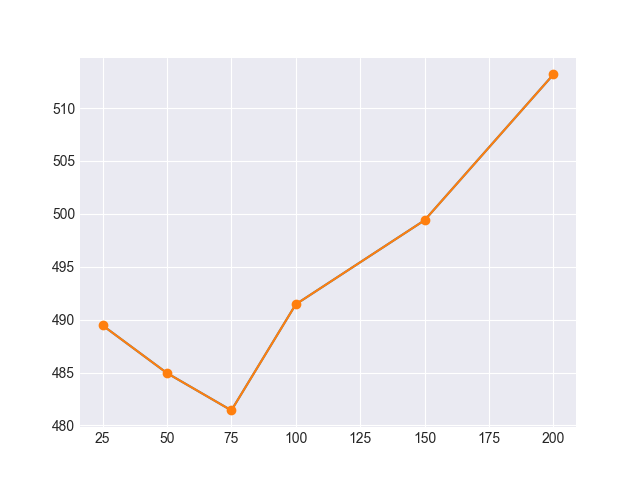
\includegraphics[width=\textwidth]{figures/lda-perplexity.png}
    \caption{The perplexity scores for the different LDA models}
    \label{fig:lda-perplexity}
\end{figure}


The data points were plotted in a 2D plot after reducing the dimensions using t-SNE.
Each data point was colored based on some trait that the specific data point had.
For the exploration of the topics, the topic with the highest probability for a given data point was used to determine the color.
A plot of this can be seen in Figure~\ref{fig:lda-dist}.
Although it might be hard to interpret as a 2D plot in this report, the bokeh \footnote{Bokeh, https://bokeh.pydata.org/en/latest/} library allowed for the generation an interactive plot.
Hovering over each data point would show the content of the report and the topics assigned to it, making it a convenient way to explore the data and the generated topics.

\begin{figure}
    \centering
    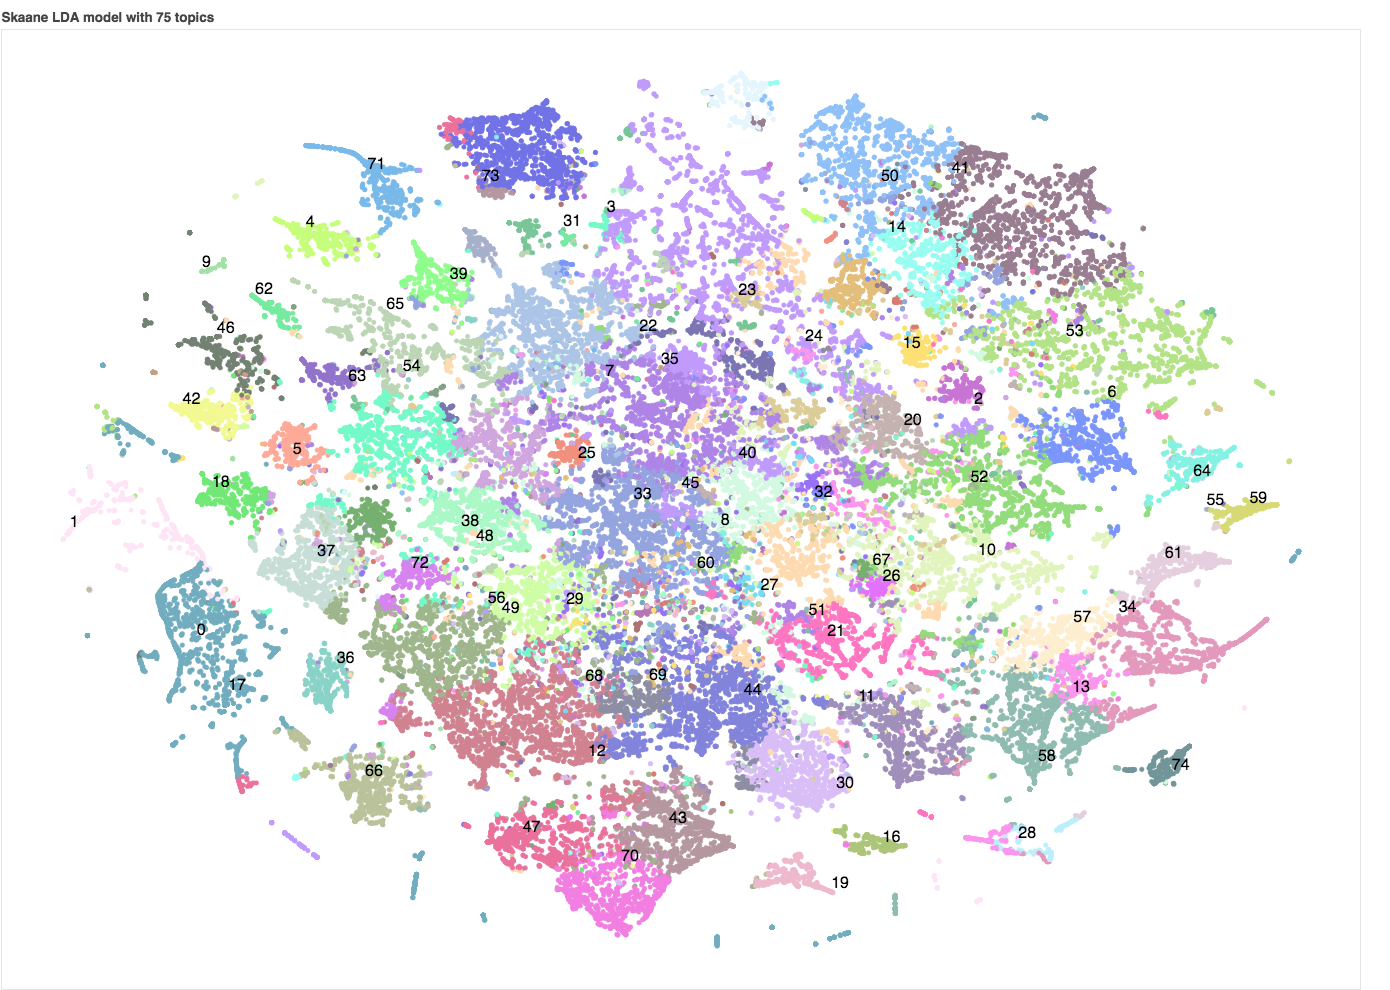
\includegraphics[width=\textwidth]{figures/lda-2d-distribution.png}
    \caption{A 2D plot of the text data, where each point is colored by topic with the highest probability}
    \label{fig:lda-dist}
\end{figure}

Samples of the generated topics can be seen in Figure~\ref{fig:topic-wordclouds}.
Another way to visualize the topics for inspection is using the LDAvis technique described by Sievert et al\@.~\cite{sievert2014ldavis}.
They propose a \textit{relevance} measure where the probability for a certain term within a topic is weighted against how common that topic is in the entire corpus.
The interactive interface provided by pyLDAvis \footnote{pyLDAvis, https://github.com/bmabey/pyLDAvis}  can be seen in Figure~\ref{fig:ldavis-sample}.
This provided a good way to explore the important words in each topic.

\begin{figure}
    \centering
    \thirdsubfigimg{wordcloud-1}{A wordcloud over the words occurring in topic 1 for a 75 topic LDA model.}
    \thirdsubfigimg{wordcloud-17}{A wordcloud over the words occurring in topic 17 for a 75 topic LDA model}
    \caption{Wordclouds for a 75 topic LDA model}
    \label{fig:topic-wordclouds}
\end{figure}

\begin{figure}
    \centering
    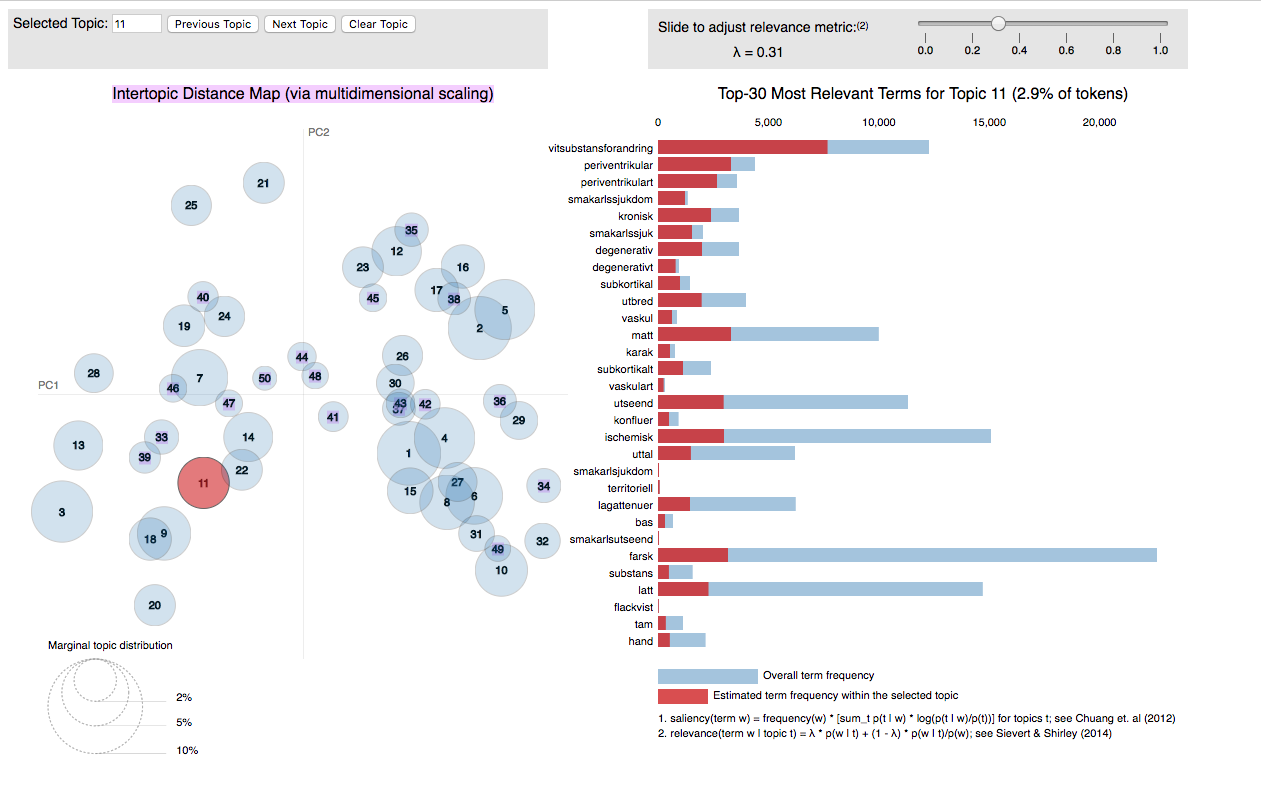
\includegraphics[width=\textwidth]{figures/ldavis-sample.png}
    \caption{A way to visualize and analyze topics based on their relevance and frequency}
    \label{fig:ldavis-sample}
\end{figure}

\section{The Relationship Between Topics and Categories}
\label{sec:topic-categories}

With the initial set of labeled reports, it was natural to explore and try to find a relationship between the initial set of categories and the inherent structure of the data.
This was done by visualizing the LDA model again.
In order to find any existing relationship between the topics and the labeled samples, the points were colored based on their assigned labels.
The color of a point in the plot was based on the first label of a sorted list of the point's labels.
Unlabeled samples were hidden from the plot.
The resulting plot can be seen in Figure~\ref{fig:categories-lda-75}.
Even if the categories are not the same in the final system, knowledge of an existing relationship might still be exploited even if the specifics change.
If there is an existing relationship between categories and topics, it is likely to remain since the new categories still aim to describe the same reports.

\begin{figure}
    \centering
    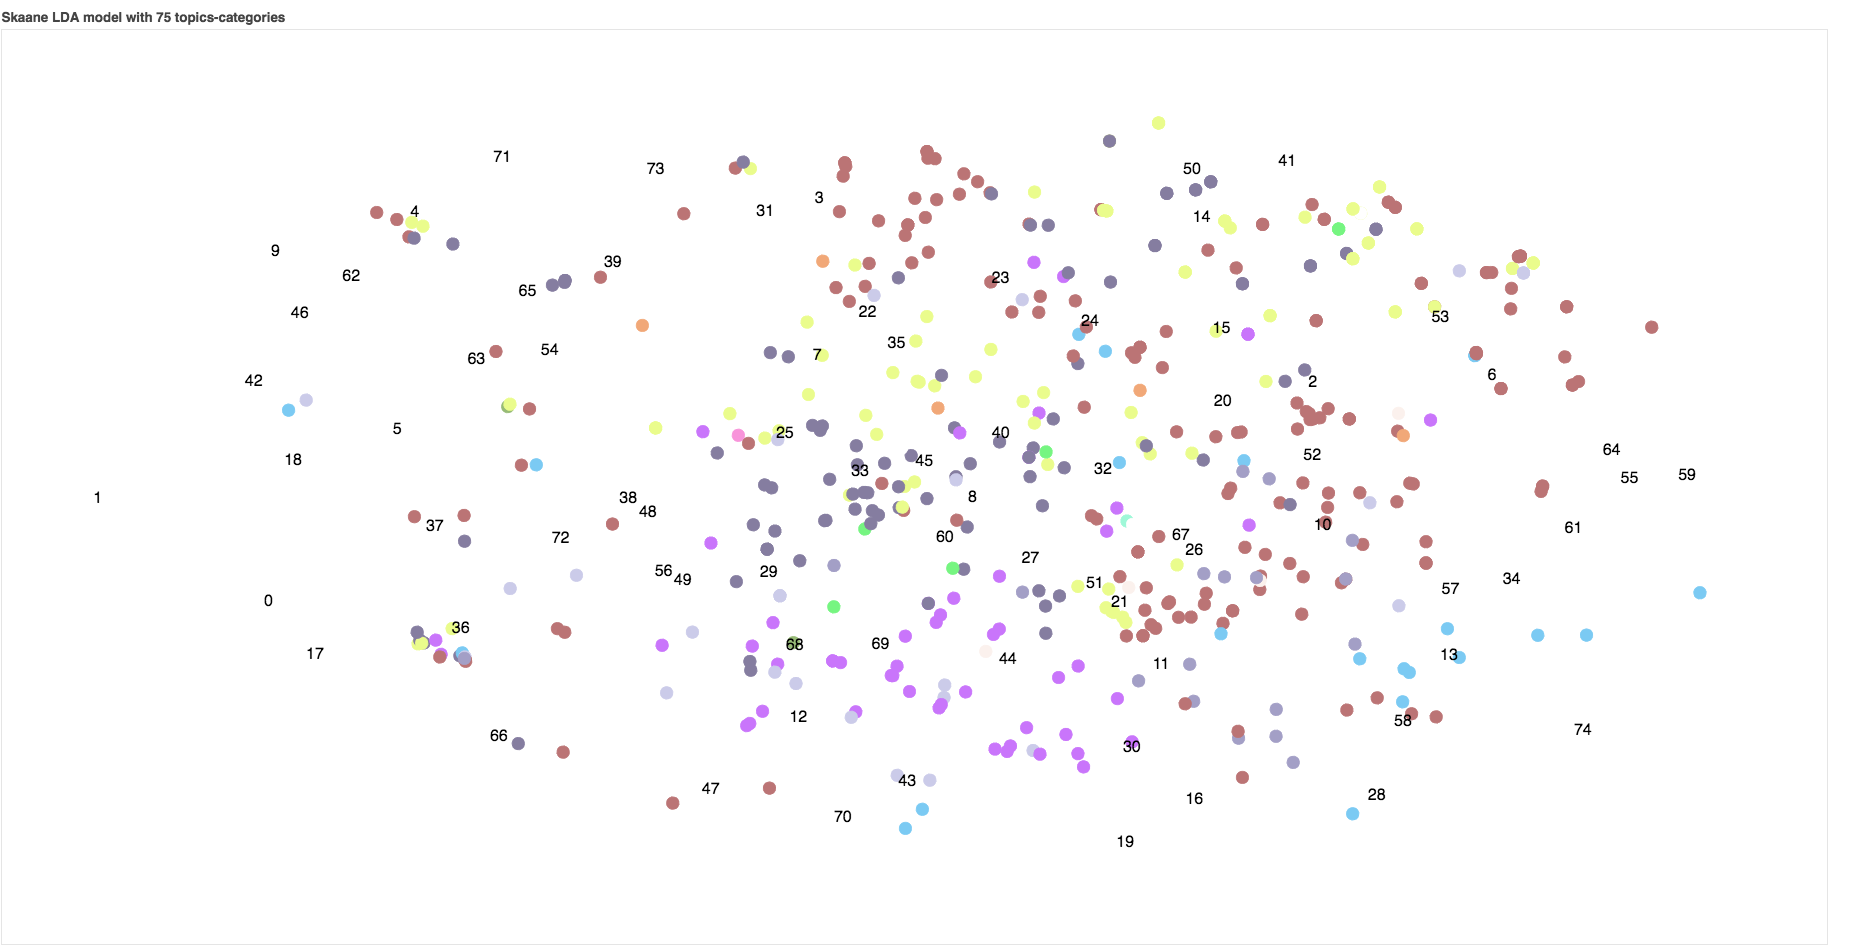
\includegraphics[width=\textwidth]{figures/categories-lda-75.png}
    \caption{The labeled data points plotted in 2D, and colored based on the first label of the report in alphabetical order.}
    \label{fig:categories-lda-75}
\end{figure}

From this plot it is clear that there is a grouping of labels.
Certain labels are more likely to occur in documents assigned a specific topic.
For example, the purple points in the lower part of the graph represents the ``blödning'' label, the gray labels in the middle represents ``infarkt'' and the light blue ones that are mostly concentrated in the bottom right corner represents ``infektion''.
It is clear that these labels are not evenly spread out over all the topics, but neither are they confined enough to make a direct mapping between topics and labels.

To explore the relationships in more detail, they can be analyzed with the help of histograms over the topics for a certain label, as well as histograms over categories that had a certain topic as its most likely topic
This was done on the 4 most common labels, since most of the others lacked the amount of reports necessary to identify a clear pattern.
In Figure~\ref{fig:category-label-distribution} the counts of most likely topics for the four most common categories are displayed.
The four most common categories were used because the others lacked the amount of reports necessary to identify a clear pattern.
These categories are ``infarkt'', ``kärlsjukdom'', ``normal'' and ``blödning''.
From the histograms it is clear that documents of a certain category are more likely to be assigned certain topics, at least in these cases.
Even though there exist a clear relationship, it is not exclusive enough to make out any clear relation.
The number of topics assigned and reports labeled for these 4 topics can be seen in Table~\ref{tab:topic-categories}.

\begin{table}
    \centering
    \begin{tabular}{|c|cc|}
        \hline
        \textbf{Label} & \textbf{No. reports} & \textbf{No. most likely topics} \\
        \hline
        Normal & 181 & 28\\
        Tumör & 29 & 15\\
        Infarkt & 105 & 27\\
        Blödning & 69 & 19\\
        Kärlsjukdom & 145 & 28\\
        Hydrocefalus & 10 & 5\\
        Demens & 14 & 9\\
        Trauma & 27 & 12\\
        Cysta & 9 & 7\\
        Missbildning & 3 & 3\\
        Inklämmning & 4 & 1\\
        Infektion & 29 & 15\\
        Syndrom & 2 & 2\\
        Metabol & 1 & 1\\
        \hline
    \end{tabular}
    \caption{The number of reports assigned a certain category, as well as the number of different topics assigned as the most likely one for reports with the given category.}
    \label{tab:topic-categories}
\end{table}

\begin{figure}[h!]
    \centering
    \thirdsubfigimg{infarkt}{The counts of most likely topics for the ``infarkt'' label.}
    \thirdsubfigimg{karlsjukdom}{The counts of most likely topics for the ``kärlsjukdom'' label.}
    \quad
    \thirdsubfigimg{normal}{The counts of most likely topics for the ``normal'' label.}
    \thirdsubfigimg{blodning}{The counts of most likely topics for the ``blödning'' label.}
    \caption{The counts of the most likely topics for the four most common categories.}
    \label{fig:category-label-distribution}
\end{figure}

In order to analyze these topics further, Figure~\ref{fig:topic-category-distribution} shows the different categories that has a certain topic assigned to it as the most likely one.
Taking into account the information from Table~\ref{tab:topic-categories}, i.e. that some categories are a lot more common than others in the labeled dataset, there is not a clear enough pattern to distinguish between different categories based on the topics.
This does not take the multi-label nature of the data into account.
If a report has multiple labels assigned to it, both of the labels are counted separately.

\begin{figure}[h!]
    \centering
    \thirdsubfigimg{categories-topic-13}{The counts categories where the most likely topic for the report was 13.}
    \thirdsubfigimg{categories-topic-16}{The counts categories where the most likely topic for the report was 16.}
    \quad
    \thirdsubfigimg{categories-topic-25}{The counts categories where the most likely topic for the report was 25.}
    \thirdsubfigimg{categories-topic-35}{The counts categories where the most likely topic for the report was 35.}
    \caption{The categories of the different reports that are assigned a certain topic as the most likely one.}
    \label{fig:topic-category-distribution}
\end{figure}

\section{The Relationship Between Topics and Invalid Reports}
\label{sec:topic-invalid}

The next step was identifying the topics that were assigned to the invalid reports.
First, topic 1 and 17 were identified as interesting based on the word distribution for them.
This was done using both the 2D plot of the data and LDAvis visualization.
The most common terms for these two topics can be seen in Figure~\ref{fig:topic-wordclouds}.

As described in Section~\ref{sec:exp3-method}, a set of reports were labeled as invalid or valid in order to evaluate the technique.
This set is split into a training set and a validation set.
In order to verify and gain further insight into how invalid reports were related to topics, the training set was used for further analysis.

\begin{figure}[h!]
    \centering
    \thirdsubfigimg{invalid_reports_most_likely_topics_histogram}{The distribution of the topics with the highest probability for the invalid reports in the training set.}
    \thirdsubfigimg{valid_reports_most_likely_topics_histogram}{The distribution of the topics with the highest probability for the valid reports in the training set.}
    \caption{Distribution over the most likely topics for the valid and invalid reports. Note that only topics that occurred at least once are shown in the histogram.}
    \label{fig:most-likely-topics}
\end{figure}

The distribution of the topics with the highest likelihood for the invalid reports in the training set can be seen in Figure~\ref{fig:most-likely-topics} (a).
A couple of topics, 1 and 17, clearly stand out as the ones that most invalid reports gets assigned.
Specifically, topic 1 had a count of 131 reports from the invalid reports in the training set, and topic 17 had 358.
Some invalid reports have topics 0, 3, 9, 16, 47, 53, 58, 61, 62 as the most likely topic.
53 is the third most common, with a count of 3.

The corresponding plot for the valid reports can be seen in Figure~\ref{fig:most-likely-topics} (b).
There is a lot more variety among the most likely topics here.
Topics 1 and 17 occur very infrequently.
Topic 1 occurs 0 times, while topic 17 occurs 2 times.
The third most common topic from the invalid reports, 53, occurs 28 times.
The ones having topic 17 had 4 and 8 prominent topics assigned to them.

Each topic that was assigned to a report with a probability above 10\% was considered to be a prominent topic.
The number of prominent topics for the invalid reports can be seen in Figure~\ref{fig:prominent-topic-dist} (a).
1, 2 and 3 number of prominent topics are the most common.
And there are barely any reports having more than 6.
The corresponding plot for the valid reports can be seen in Figure~\ref{fig:prominent-topic-dist} (b).
In the case of valid reports, 6 is the most common number of prominent topics. 
The topics are a lot more spread out than in the case of the invalid reports.

\begin{figure}[h!]
    \centering
    \thirdsubfigimg{invalid_reports_prominent_topics_count_histogram}{The distribution of the number of prominent topics assigned to the invalid reports in the training set.}
    \thirdsubfigimg{valid_reports_prominent_topics_count_histogram}{The distribution of the number of prominent topics assigned to the valid reports in the training set.}
    \caption{The distribution of the number of prominent topics for the two categories.}
    \label{fig:prominent-topic-dist}
\end{figure}

Another idea was to evaluate whether or not 17 and 1 were among the most probable topics for the reports.
A simple evaluation of this on the set of valid reports showed that it was not a good approach.
For example, seeing if 17 or 1 had more than 10\% probability returned 48 and 45 valid reports, respectively.
Checking if both were above the threshold returned 11 reports.